\documentclass[letterpaper,12pt]{article}

\usepackage[utf8]{inputenc}
\usepackage[T1]{fontenc}
\usepackage[english]{babel}
\usepackage{lmodern}
\usepackage{geometry}
\usepackage{amsmath,amssymb,mathtools}
\usepackage{graphicx}
\usepackage{booktabs}
\usepackage{array}
\usepackage{xcolor}
\usepackage{listings}
\usepackage{caption}
\usepackage{float}
\usepackage{placeins}
\usepackage{enumitem}
\usepackage{microtype}
\usepackage{hyperref}
\usepackage[nameinlink,noabbrev]{cleveref}

\geometry{margin=1in,letterpaper}
\graphicspath{{figures/}{../PR_LAB1/img/}}

\definecolor{udgblue}{RGB}{0,77,122}
\definecolor{codeblue}{RGB}{20,70,140}
\definecolor{codegreen}{RGB}{25,115,65}
\definecolor{codegray}{RGB}{95,95,95}
\definecolor{codebg}{RGB}{247,248,250}

\hypersetup{
    colorlinks=true,
    linkcolor=blue,
    citecolor=blue,
    filecolor=magenta,
    urlcolor=blue,
    pdftitle={Differential-Drive Robot Simulation and Dead-Reckoning Localization},
    pdfauthor={Diego Marzá Fuertes and Mario López Honrubia}
}

\lstdefinestyle{pythonstyle}{
    language=Python,
    basicstyle=\ttfamily\small,
    keywordstyle=\color{codeblue}\bfseries,
    commentstyle=\color{codegreen},
    stringstyle=\color{orange!70!black},
    numbers=left,
    numberstyle=\scriptsize\color{codegray},
    stepnumber=1,
    numbersep=8pt,
    backgroundcolor=\color{codebg},
    frame=single,
    rulecolor=\color{black!15},
    breaklines=true,
    showstringspaces=false,
    tabsize=4,
    columns=fullflexible,
    keepspaces=true
}
\lstset{style=pythonstyle}

\newcommand{\R}{\mathbb{R}}
\newcommand{\opluspose}{\mathbin{\oplus}}
\newcommand{\ominuspose}{\mathbin{\ominus}}

\begin{document}

\title{Differential Drive Mobile Robot Simulation and Dead Reckoning}
\author{Diego Marzá Fuertes and Mario López Honrubia}
\date{October 2026}
\maketitle

\begin{abstract}
This report presents the implementation and validation of a differential-drive
mobile robot simulator and a dead-reckoning localization method. Planar direct
and inverse pose compounding were first implemented and incorporated into the
simulation and localization modules. Lab 1 implements the planar motion model
and the simulated encoder and compass measurements. Lab 2 converts the encoder
readings into body motion and integrates them to estimate the robot pose through
dead reckoning. Circular and figure-eight trajectories are used to compare
different velocity gains and encoder-noise levels. The results show that the
tested gains produce similar long-term paths, whereas increasing the encoder
noise causes increasing localization drift.
\end{abstract}

\section{Introduction}

The objective of Labs 1 and 2 is to build the simulation and odometric
localization foundations required by the later probabilistic localization
exercises. The Pre-Lab covered the planar pose representation and the direct
and inverse pose-compounding operators. Lab 1 then applied these operations to
the differential-drive simulator, wheel-encoder model, and commanded
trajectories. Lab 2 used the simulated encoder readings to estimate the robot
pose through dead reckoning.

The implementation uses a world frame, denoted by $N$, and a body-fixed robot
frame, denoted by $B$. A planar robot pose contains two Cartesian coordinates
and one yaw angle. Lab 1 produces the simulated or ground-truth state, whereas
Lab 2 reconstructs the pose using only incremental encoder information.

The report is organized accordingly. The remainder of this introduction
describes the software structure and the Pre-Lab pose operations.
\Cref{sec:simulation} presents the differential-drive simulation, and
\cref{sec:dead-reckoning} describes the dead-reckoning implementation.
The experimental comparison is discussed in \cref{sec:results}, followed by
the conclusions in \cref{sec:conclusions}.

\subsection{Development environment and software structure}

Jupyter Notebook was used only in Lab 0 to implement and validate the direct
and inverse pose-compounding operations, $\oplus$ and $\ominus$. These
operations were subsequently incorporated into the Python modules used in
Labs 1 and 2. NumPy provides vector and matrix operations, Matplotlib is used
for visualization, and Robotics Toolbox supplies the animated vehicle
representation.

The relevant software components and their roles are summarized in
\cref{tab:classes}.

\begin{table}[H]
    \centering
    \caption{Main Python files used in Labs 1 and 2.}
    \label{tab:classes}
    \small
    \renewcommand{\arraystretch}{1.08}
    \begin{tabular}{p{0.42\textwidth}p{0.50\textwidth}}
        \toprule
        File & Responsibility\\
        \midrule
        \texttt{Pose3D.py} & Represents a planar pose and implements direct and inverse pose compounding.\\
        \texttt{SimulatedRobot.py} & Defines the common simulation interface, state storage and visualization infrastructure.\\
        \texttt{DifferentialDriveSimulatedRobot.py} & Implements the differential-drive motion model and simulated sensors.\\
        \texttt{Localization.py} & Provides the iterative localization loop and trajectory visualization.\\
        \texttt{DR\_3DOFDifferentialDrive.py} & Converts encoder readings into body motion and performs dead-reckoning integration.\\
        \texttt{main.py} & Configures the map and initial state, creates the simulated and dead-reckoning robots, and runs the localization sequence.\\
        \bottomrule
    \end{tabular}
\end{table}

\subsection{Pre-Lab: Planar pose operations}
\label{sec:prelab}

\subsubsection{Planar pose representation}

A three-degree-of-freedom pose is represented by
\begin{equation}
    \boldsymbol{\eta}=
    \begin{bmatrix}x&y&\psi\end{bmatrix}^{T}\in\R^{3},
\end{equation}
where $(x,y)$ is the position and $\psi$ is the yaw angle. Its equivalent
homogeneous transformation is
\begin{equation}
    T(\boldsymbol{\eta})=
    \begin{bmatrix}
        \cos\psi & -\sin\psi & x\\
        \sin\psi &  \cos\psi & y\\
        0 & 0 & 1
    \end{bmatrix}.
    \label{eq:pose-transform}
\end{equation}
This matrix form explains the pose operations used throughout the simulator:
direct compounding corresponds to multiplying transformations, and inverse
compounding corresponds to inverting a transformation.

\subsubsection{Direct pose compounding}

Let ${}^{A}\boldsymbol{x}_{B}$ describe frame $B$ relative to frame $A$, and
let ${}^{B}\boldsymbol{x}_{C}$ describe frame $C$ relative to $B$. The pose of
$C$ relative to $A$ is
\begin{equation}
    {}^{A}\boldsymbol{x}_{C}
    ={}^{A}\boldsymbol{x}_{B}\opluspose{}^{B}\boldsymbol{x}_{C},
\end{equation}
which is equivalent to
$T({}^{A}\boldsymbol{x}_{C})=T({}^{A}\boldsymbol{x}_{B})
T({}^{B}\boldsymbol{x}_{C})$. In coordinate form,
\begin{equation}
\begin{bmatrix}
{}^{A}x_C\\{}^{A}y_C\\{}^{A}\psi_C
\end{bmatrix}
=
\begin{bmatrix}
{}^{A}x_B+{}^{B}x_C\cos({}^{A}\psi_B)-{}^{B}y_C\sin({}^{A}\psi_B)\\
{}^{A}y_B+{}^{B}x_C\sin({}^{A}\psi_B)+{}^{B}y_C\cos({}^{A}\psi_B)\\
{}^{A}\psi_B+{}^{B}\psi_C
\end{bmatrix}.
\label{eq:oplus}
\end{equation}

The $\oplus$ operator is used to compose poses or motions expressed in
different reference frames. In this case, ${}^{B}\boldsymbol{x}_{C}$ cannot be
added directly to ${}^{A}\boldsymbol{x}_{B}$ because its components are written
in frame $B$. The operation first transforms them into frame $A$ and then
combines both poses to obtain ${}^{A}\boldsymbol{x}_{C}$.

The implementation extracts the pose components, evaluates
\cref{eq:oplus}, and returns another \texttt{Pose3D} object. The essential
operation is:
\begin{lstlisting}[caption={Core of the direct compounding implementation.}]
x_result = xB + xC * cos(theta_B) - yC * sin(theta_B)
y_result = yB + xC * sin(theta_B) + yC * cos(theta_B)
theta_result = theta_B + theta_C
return Pose3D(np.array([[x_result], [y_result], [theta_result]]))
\end{lstlisting}

\subsubsection{Inverse pose compounding}

Inverse compounding expresses frame $A$ relative to frame $B$ from the pose of
$B$ relative to $A$:
\begin{equation}
{}^{B}\boldsymbol{x}_{A}=\ominuspose{}^{A}\boldsymbol{x}_{B}
=
\begin{bmatrix}
-{}^{A}x_B\cos({}^{A}\psi_B)-{}^{A}y_B\sin({}^{A}\psi_B)\\
 {}^{A}x_B\sin({}^{A}\psi_B)-{}^{A}y_B\cos({}^{A}\psi_B)\\
-{}^{A}\psi_B
\end{bmatrix}.
\label{eq:ominus}
\end{equation}
This is the coordinate form of
$T({}^{B}\boldsymbol{x}_{A})=T({}^{A}\boldsymbol{x}_{B})^{-1}$.

The implementation evaluates \cref{eq:ominus} directly and returns the inverse
pose as another \texttt{Pose3D} object:
\begin{lstlisting}[caption={Core of the inverse compounding implementation.}]
x_result = -xB * cos(theta_B) - yB * sin(theta_B)
y_result =  xB * sin(theta_B) - yB * cos(theta_B)
theta_result = -theta_B
return Pose3D(np.array([[x_result], [y_result], [theta_result]]))
\end{lstlisting}

After implementing and testing both operators in the Pre-Lab notebook, the
same code was included in \texttt{Pose3D.py}. This makes $\oplus$ and $\ominus$
available as \texttt{Pose3D} methods for the differential-drive simulation
developed in Lab 1.

\section{Lab 1: Simulation}
\label{sec:simulation}

Lab 1 consists of completing the \texttt{DifferentialDriveSimulatedRobot}
class, which inherits from \texttt{SimulatedRobot}. The base class provides the
common simulation interface, state storage, and visualization tools, whereas
the derived class implements the differential-drive motion and sensor models.

\subsection{\texttt{\_\_init\_\_}: robot configuration}

The constructor first calls \texttt{super().\_\_init\_\_} to initialise the
state, map, sampling period, and visualization variables provided by
\texttt{SimulatedRobot}. The simulated state contains the world-frame pose and
body-frame velocity:
\begin{equation}
    \boldsymbol{x}_{s,k}=
    \begin{bmatrix}
        \boldsymbol{\eta}_{s,k}\\
        \boldsymbol{\nu}_{s,k}
    \end{bmatrix}
    =
    \begin{bmatrix}
        x_k&y_k&\psi_k&u_k&v_k&r_k
    \end{bmatrix}^{T}.
\end{equation}

It then defines the parameters required by the differential-drive model. The
wheel separation is $b=0.5$~m, the wheel radius is $R=0.1$~m, and the simulator
initially assigns $N_p=1024$ encoder pulses per wheel revolution. However,
\texttt{main.py} creates the dead-reckoning object before starting the
localization loop. Its constructor changes
\texttt{robot.pulse\_x\_wheelTurns} to 4096 on the same shared robot object.
Therefore, the effective resolution throughout the executed simulation is
$N_p=4096$ pulses per wheel revolution; 1024 is only the simulator's initial
default value. The motion and encoder noise are described by
\begin{equation}
    Q_s=\operatorname{diag}\left(0.1^2,\,0.01^2,\,
    \operatorname{deg2rad}(1)^2\right),\qquad
    R_e=\operatorname{diag}(22^2,22^2).
\end{equation}
Here, $Q_s$ is the covariance of the acceleration perturbation applied by the
motion model, while $R_e$ is the covariance of the encoder noise in squared
pulses. The remaining constructor parameters configure sensors that are not
required for the simulation and dead-reckoning tasks discussed here.

\subsection{\texttt{fs}: motion model}

This method computes the new simulated state from the previous state and the
commanded forward and angular velocities. The desired input is
$\boldsymbol{u}_{s,k}=[u_d,\,r_d]^{T}$. Because a differential-drive robot
cannot move laterally, the corresponding desired body velocity is
$\boldsymbol{\nu}_d=[u_d,\,0,\,r_d]^{T}$.

\begin{figure}[H]
    \centering
    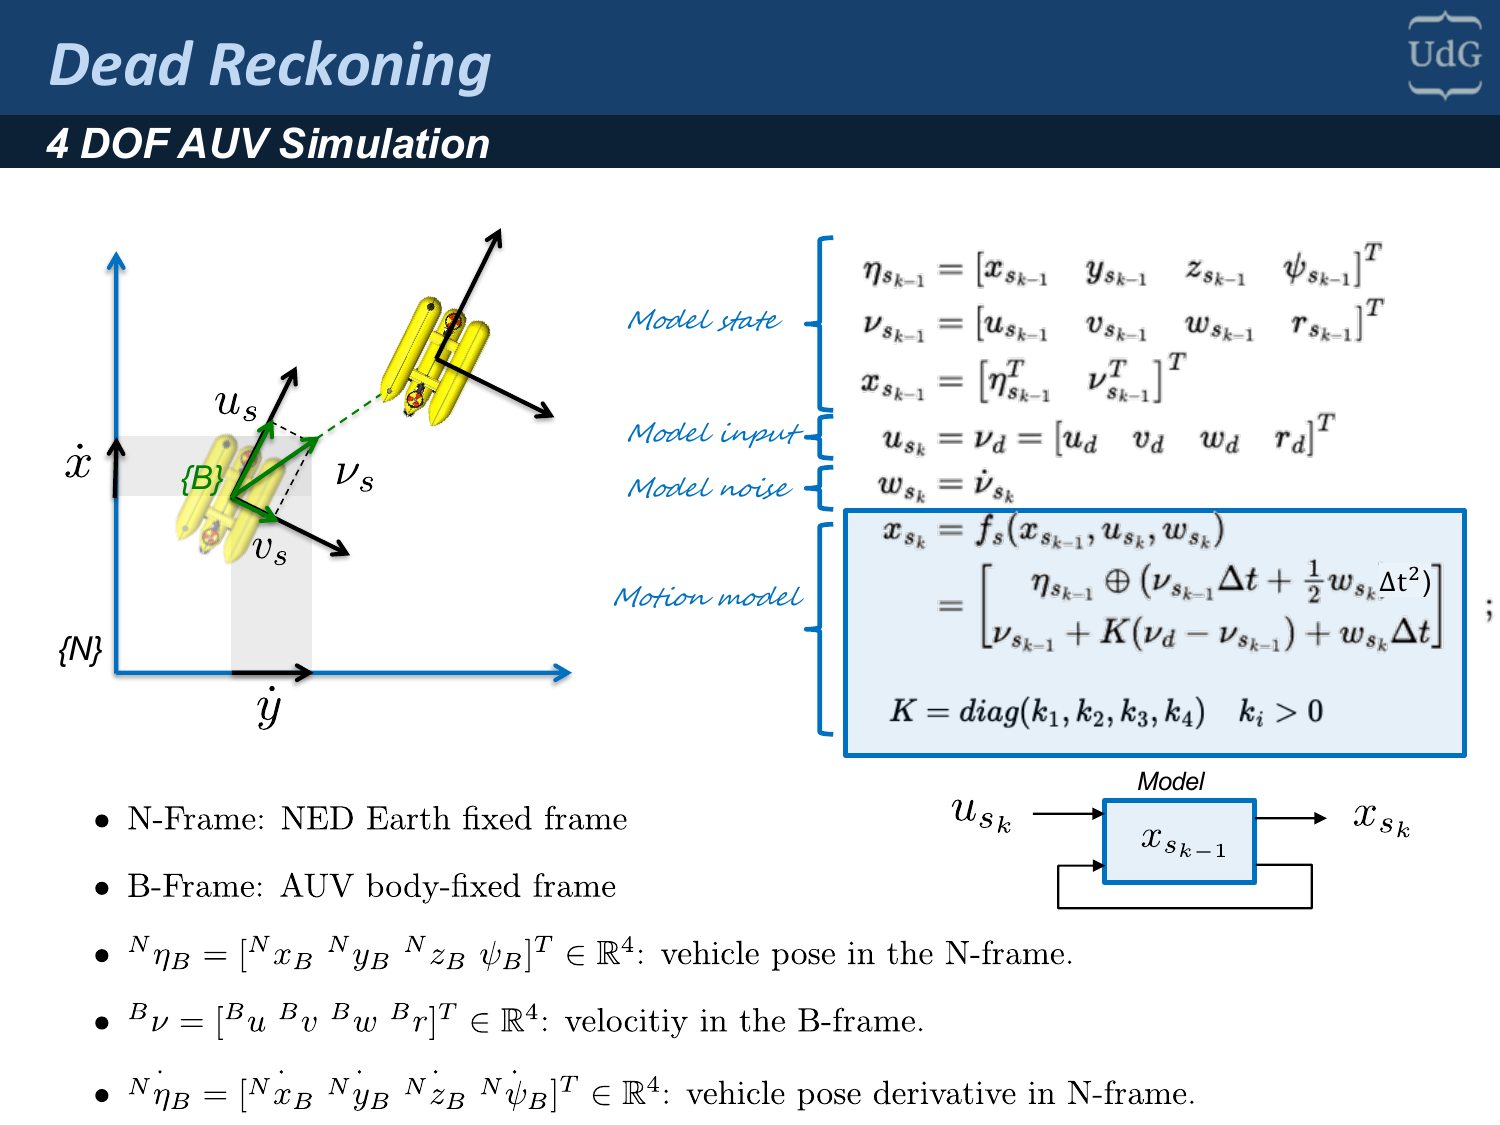
\includegraphics[trim=0pt 170pt 0pt 90pt,clip,
    width=\textwidth]{fs_motion_model_slide.png}
    \caption{State, input, noise, and motion model used by \texttt{fs}.}
    \label{fig:fs-model}
\end{figure}

The planar version of the model in \cref{fig:fs-model} uses
$\boldsymbol{\eta}=[x,\,y,\,\psi]^T$ and
$\boldsymbol{\nu}=[u,\,v,\,r]^T$, with $v_d=0$ because the wheels prevent
lateral motion.

The nominal implementation uses $K=I_3$. Its effect on the velocity response
is discussed in \cref{sec:results}.

The key lines in \texttt{fs} are therefore:
\begin{lstlisting}[caption={Pose and velocity update in the simulator.}]
w = np.random.multivariate_normal(np.zeros(3), self.Qsk).reshape(3, 1)
eta_new = eta_prev.oplus(Pose3D(
    nu_prev * self.dt + 0.5 * w * self.dt**2))
nu_new = nu_prev + K @ (nu_desired - nu_prev) + w * self.dt
\end{lstlisting}

\subsection{\texttt{ReadEncoders}: wheel-encoder simulation}

\texttt{ReadEncoders} converts the motion between two consecutive simulated
poses into the measurements that would be produced by the left and right wheel
encoders. The implemented sequence is summarized in \cref{fig:encoder-flow}.

\begin{figure}[H]
    \centering
    \small
    \begin{tabular}{c}
        \fbox{\parbox{0.82\textwidth}{\centering
        \textbf{1. Relative motion in the previous body frame}\\[-0.1em]
        $\displaystyle
        \Delta\boldsymbol{\eta}_k=
        (\ominuspose\boldsymbol{\eta}_{s,k-1})
        \opluspose\boldsymbol{\eta}_{s,k}$}}\\[0.25em]
        $\downarrow$\\[0.25em]
        \fbox{\parbox{0.82\textwidth}{\centering
        \textbf{2. Extract the local forward displacement and yaw change}\\[-0.1em]
        $\displaystyle d=\Delta x_k,\qquad
        \Delta\psi=\Delta\psi_k$}}\\[0.25em]
        $\downarrow$\\[0.25em]
        \fbox{\parbox{0.82\textwidth}{\centering
        \textbf{3. Compute the distance traveled by each wheel}\\[-0.1em]
        $\displaystyle d_L=d-\frac{b}{2}\Delta\psi,\qquad
        d_R=d+\frac{b}{2}\Delta\psi$}}\\[0.25em]
        $\downarrow$\\[0.25em]
        \fbox{\parbox{0.82\textwidth}{\centering
        \textbf{4. Convert wheel distances into ideal encoder pulses}\\[-0.1em]
        $\displaystyle
        \boldsymbol{z}_{\mathrm{ideal}}=
        \frac{N_p}{2\pi R}
        \begin{bmatrix}d_L\\d_R\end{bmatrix}$}}\\[0.25em]
        $\downarrow$\\[0.25em]
        \fbox{\parbox{0.82\textwidth}{\centering
        \textbf{5. Add encoder noise and form the measurement}\\[-0.1em]
        $\displaystyle
        \boldsymbol{\epsilon}_k\sim\mathcal{N}(\boldsymbol{0},R_e),\qquad
        \boldsymbol{z}_{s,k}=\boldsymbol{z}_{\mathrm{ideal}}+
        \boldsymbol{\epsilon}_k$}}
    \end{tabular}
    \caption{Sequence implemented by \texttt{ReadEncoders}.}
    \label{fig:encoder-flow}
\end{figure}

The use of $\ominus$ in the first step is essential. Both simulated poses are
stored relative to the world frame, but an encoder measures the displacement
in the robot frame. In transformation form, the required relative motion is
\begin{equation}
    T(\Delta\boldsymbol{\eta}_k)=
    T(\boldsymbol{\eta}_{s,k-1})^{-1}
    T(\boldsymbol{\eta}_{s,k}).
\end{equation}
The inverse operator removes the previous world-frame pose, and the following
$\oplus$ expresses the current pose relative to that previous robot frame. A
direct subtraction would not rotate the translational displacement into the
body axes and would therefore give incorrect wheel motion when the robot is
not aligned with the world frame.

For the executed experiment, $b=0.5$~m, $R=0.1$~m, and the effective encoder
resolution is $N_p=4096$ pulses per wheel revolution. Since
\texttt{ReadEncoders} accesses the shared robot attribute after it has been
updated, this is also the value used to generate the simulated pulses. The
encoder covariance is $R_e=\operatorname{diag}(22^2,22^2)$~pulses$^2$. The
method returns $(\boldsymbol{z}_{s,k},R_e)$, where
$\boldsymbol{z}_{s,k}=[n_L,n_R]^T$ contains the noisy left and right encoder
pulses and $R_e$ describes their measurement uncertainty.

\subsection{Compass and robot visualization}

\texttt{ReadCompass} adds zero-mean Gaussian noise to the true yaw and returns
the resulting measurement together with its variance. \texttt{PlotRobot}
updates the vehicle icon using the current simulated pose.

\begin{lstlisting}[caption={Essential compass and visualization operations.}]
yaw_true = self.xsk[2, 0]
yaw_measured = yaw_true + np.random.normal(0.0, self.v_yaw_std)
return yaw_measured, self.v_yaw_std**2

self.vehicleIcon.update([self.xsk[0], self.xsk[1], self.xsk[2]])
plt.pause(0.0000001)
\end{lstlisting}

\subsection{Trajectory commands}

The simulator is tested with a constant forward speed and opposite angular
velocities. The first command produces circular motion; changing the angular
velocity sign produces the second lobe of the requested figure-eight sequence.
Each command is applied for approximately one complete revolution,
$k_{\mathrm{steps}}=\operatorname{round}(2\pi/(0.03\Delta t))=2094$. The
applied commands are $(u_d,r_d)=(0.5,0.03)$ and $(0.5,-0.03)$.
The second command starts from the final simulated state of the first, preserving
continuity between the two trajectory segments.

\begin{figure}[H]
    \centering
    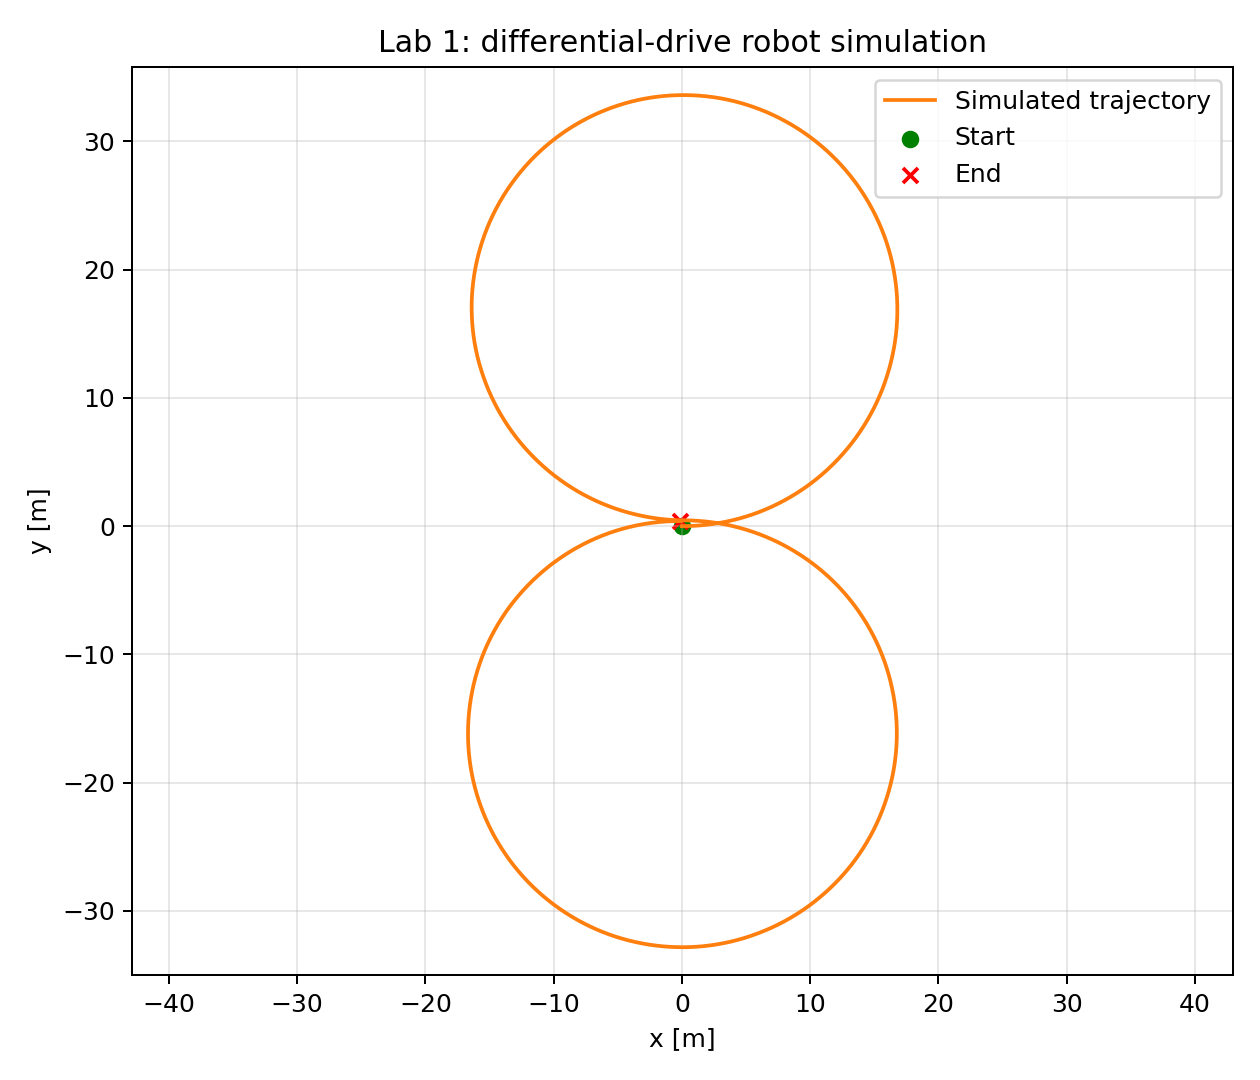
\includegraphics[width=0.48\textwidth]{simulated_robot_trajectory.png}
    \caption{Trajectory generated directly by the simulated robot for the two
    opposite angular-velocity commands.}
    \label{fig:simulated-trajectory}
\end{figure}

\section{Lab 2: Dead-Reckoning Localization}
\label{sec:dead-reckoning}

\subsection{Localisation sequence}

The \texttt{Localization} base class defines the common iterative procedure.
At every time step it:
\begin{enumerate}[label=\arabic*.]
    \item advances the simulated robot through \texttt{robot.fs};
    \item obtains the encoder-derived input through \texttt{GetInput};
    \item updates the pose estimate through \texttt{Localize}; and
    \item plots the estimated trajectory.
\end{enumerate}
The derived \texttt{DR\_3DOFDifferentialDrive} class supplies the two
algorithm-specific methods in steps 2 and 3.

\subsection{\texttt{GetInput}: encoder readings to body motion}

The template documentation describes the input both as the raw encoder vector
$[n_L,n_R]^T$ and as a generic four-component velocity. Neither is the value
that \texttt{Localize} ultimately requires in this planar implementation.
\texttt{GetInput} therefore reads $[n_L,n_R]^T$ from the simulated robot and
converts it into the three-component body velocity
$\boldsymbol{u}_k=\boldsymbol{\nu}_k=[u_k,0,r_k]^T$.

\begin{figure}[H]
    \centering
    \begin{tabular}{c}
        \fbox{\parbox{0.82\textwidth}{\centering
        \textbf{1. Read the wheel encoders}\\[-0.1em]
        $\displaystyle
        \boldsymbol{z}_{s,k}=\begin{bmatrix}n_L&n_R\end{bmatrix}^{T}$}}\\[0.25em]
        $\downarrow$\\[0.25em]
        \fbox{\parbox{0.82\textwidth}{\centering
        \textbf{2. Convert pulses into wheel distances}\\[-0.1em]
        $\displaystyle
        d_L=n_L\frac{2\pi R}{N_p},\qquad
        d_R=n_R\frac{2\pi R}{N_p}$}}\\[0.25em]
        $\downarrow$\\[0.25em]
        \fbox{\parbox{0.82\textwidth}{\centering
        \textbf{3. Recover the robot displacement}\\[-0.1em]
        $\displaystyle
        d=\frac{d_L+d_R}{2},\qquad
        \Delta\psi=\frac{d_R-d_L}{b}$}}\\[0.25em]
        $\downarrow$\\[0.25em]
        \fbox{\parbox{0.82\textwidth}{\centering
        \textbf{4. Return the planar body velocity}\\[-0.1em]
        $\displaystyle
        \boldsymbol{u}_k=
        \begin{bmatrix}u_k\\v_k\\r_k\end{bmatrix}
        =\begin{bmatrix}d/\Delta t\\0\\\Delta\psi/\Delta t\end{bmatrix}$}}
    \end{tabular}
    \caption{Conversion performed by \texttt{GetInput}.}
    \label{fig:get-input-flow}
\end{figure}

The zero lateral component represents the non-holonomic constraint of the
differential-drive platform. The implementation uses the same effective
resolution, $N_p=4096$ pulses per wheel revolution, to convert the measurements
back into wheel distances. It also uses $R=0.1$~m, $b=0.5$~m, and
$\Delta t=0.1$~s.

\subsection{Dead-reckoning pose update}

The estimator integrates the encoder-derived velocity over one sampling
period and compounds that body-frame displacement with the previous estimate:
\begin{equation}
    \widehat{\boldsymbol{\eta}}_k
    =\widehat{\boldsymbol{\eta}}_{k-1}
    \opluspose
    \left(\boldsymbol{\nu}_k\Delta t\right).
    \label{eq:dead-reckoning}
\end{equation}
The multiplication by $\Delta t$ converts velocity into a local pose
increment. The $\oplus$ operation then rotates its translation according to
the previous heading before updating the world-frame pose. The complete method
is:
\begin{lstlisting}[caption={Complete \texttt{Localize} implementation.}]
def Localize(self, xk_1, uk):
    self.etak_1 = xk_1
    self.uk = uk
    nu_k = uk

    etak = Pose3D(xk_1).oplus(nu_k * self.dt)
    return etak
\end{lstlisting}
No compass, landmark or absolute-position measurement is used in this update.
Consequently, every encoder error is integrated into the next pose and cannot
be removed by the estimator.

\section{Results and discussion}
\label{sec:results}

The comparisons use the same figure-eight command with 2094 steps per turn.
Only the parameter indicated in each test is changed.

\subsection{Effect of the velocity gain}

$K$ is the feedback gain that corrects the difference between the current and
commanded body velocities through
$K(\boldsymbol{\nu}_d-\boldsymbol{\nu}_{s,k-1})$. It therefore controls how
quickly the simulated robot responds to a new command. With $K=kI_3$, a value
below one applies only part of the required correction, $k=1$ applies it in one
step, and a value above one overshoots the command before settling.

The test uses $k=0.25$, $0.5$, $1$, and $1.5$, while the encoder noise remains
at its nominal value of 22 pulses. For each value,
\cref{fig:gain-trajectories} shows the first turn and the complete figure-eight.

\begin{figure}[H]
    \centering
    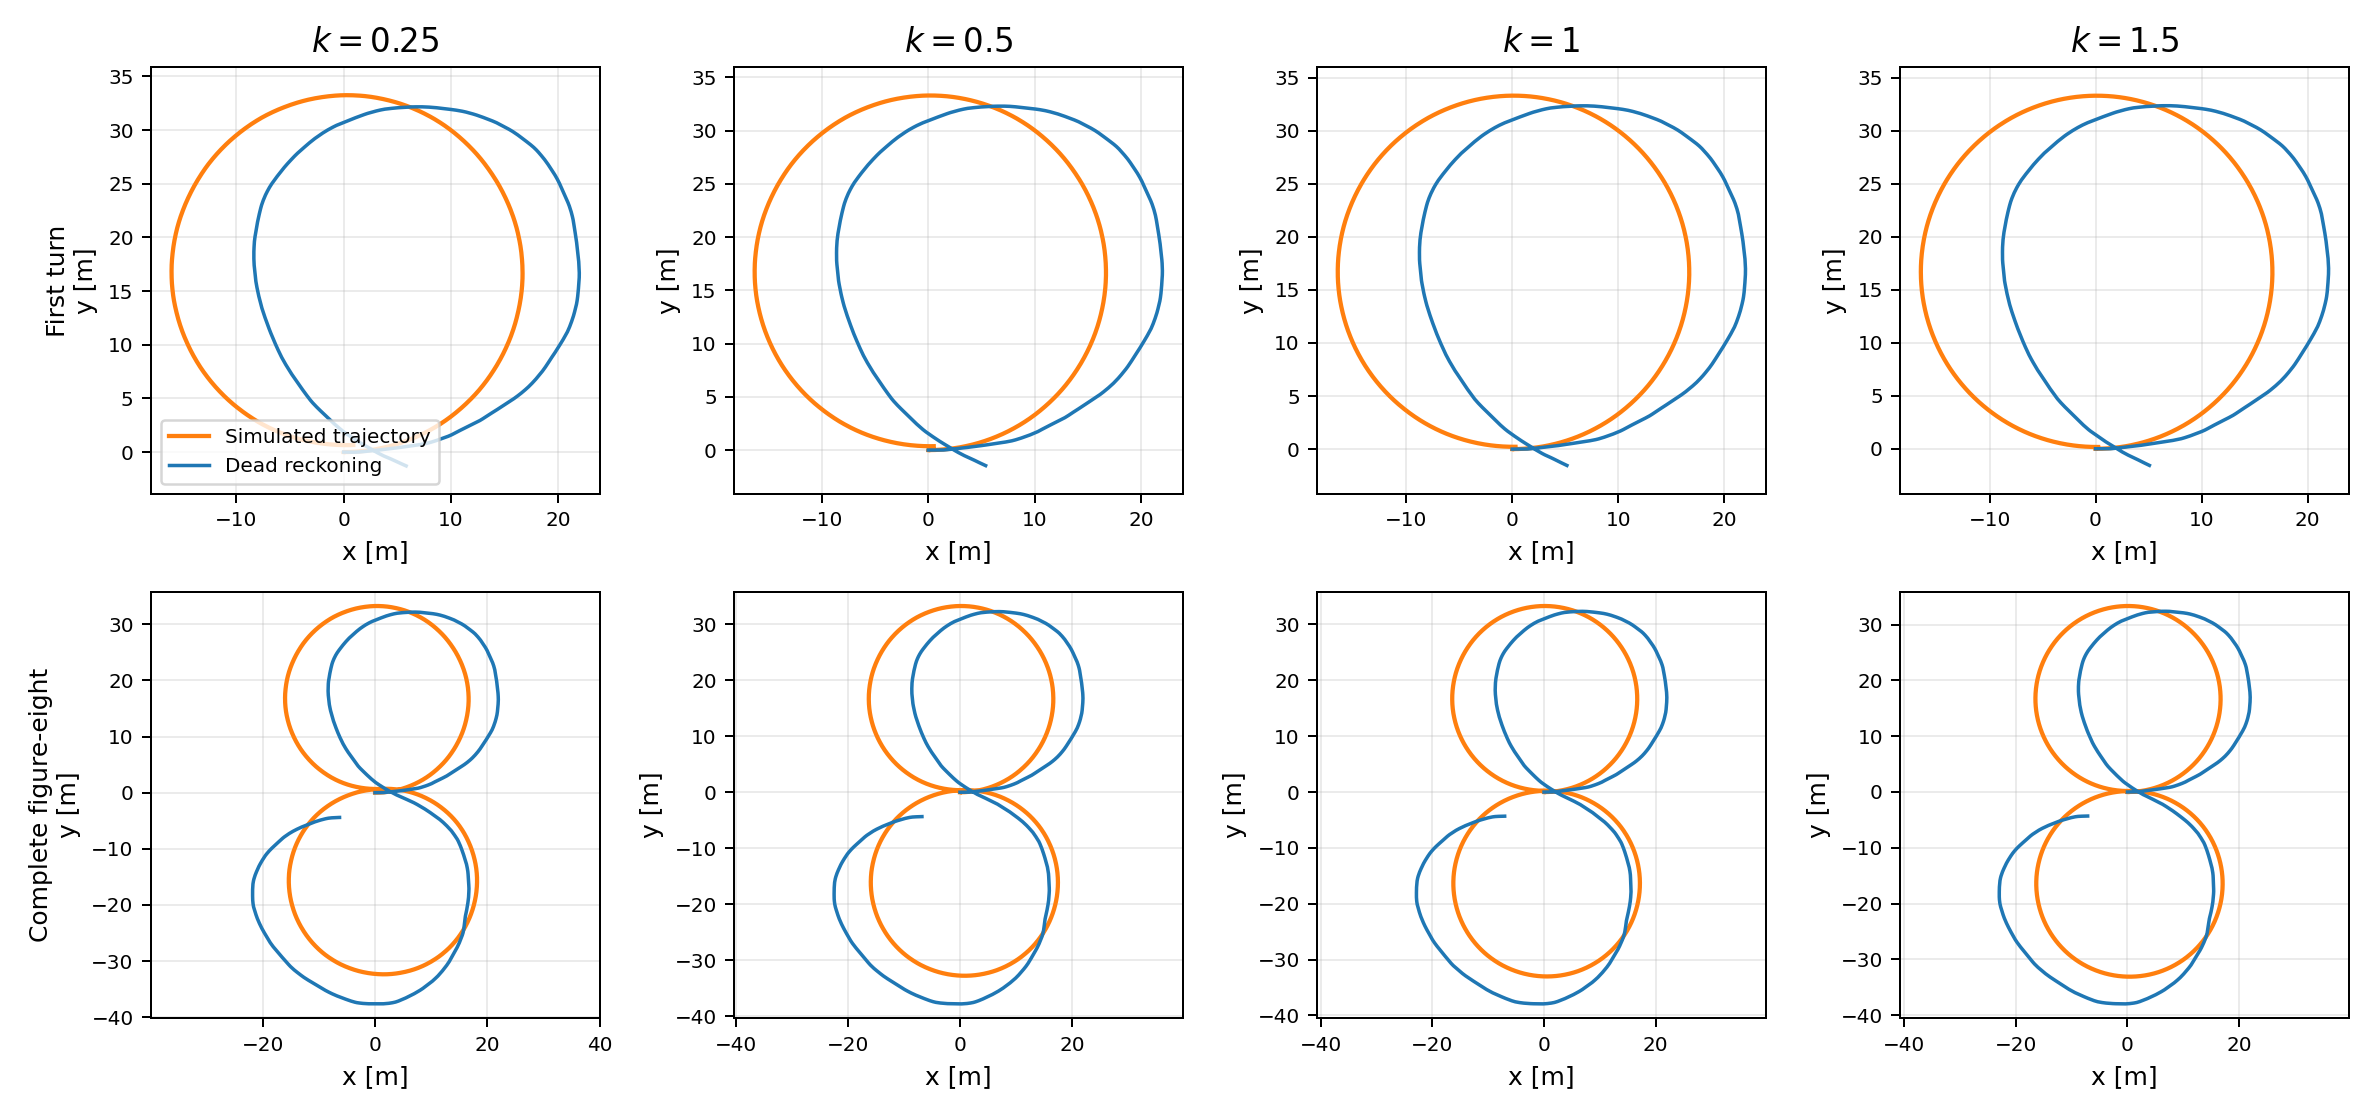
\includegraphics[width=0.94\textwidth]{gain_trajectory_comparison.png}
    \caption{Simulated and dead-reckoning trajectories for the four tested
    velocity gains.}
    \label{fig:gain-trajectories}
\end{figure}

The tested gains produce similar trajectories because the velocity transient
is short compared with the complete motion. Therefore, $K=I_3$ is retained as
the simplest direct response.

\subsection{Effect of the encoder noise}

The second test fixes $K=I_3$ and repeats both trajectories with
$\sigma_e=0$, 11, 22, and 44 pulses. Here, $\sigma_e$ is the standard
deviation of the additive encoder noise. The nominal value of 22 pulses comes
from the default covariance $R_e=\operatorname{diag}(22^2,22^2)$; it is a
noise parameter rather than the encoder resolution of $N_p=4096$ pulses per
wheel revolution.

\begin{figure}[H]
    \centering
    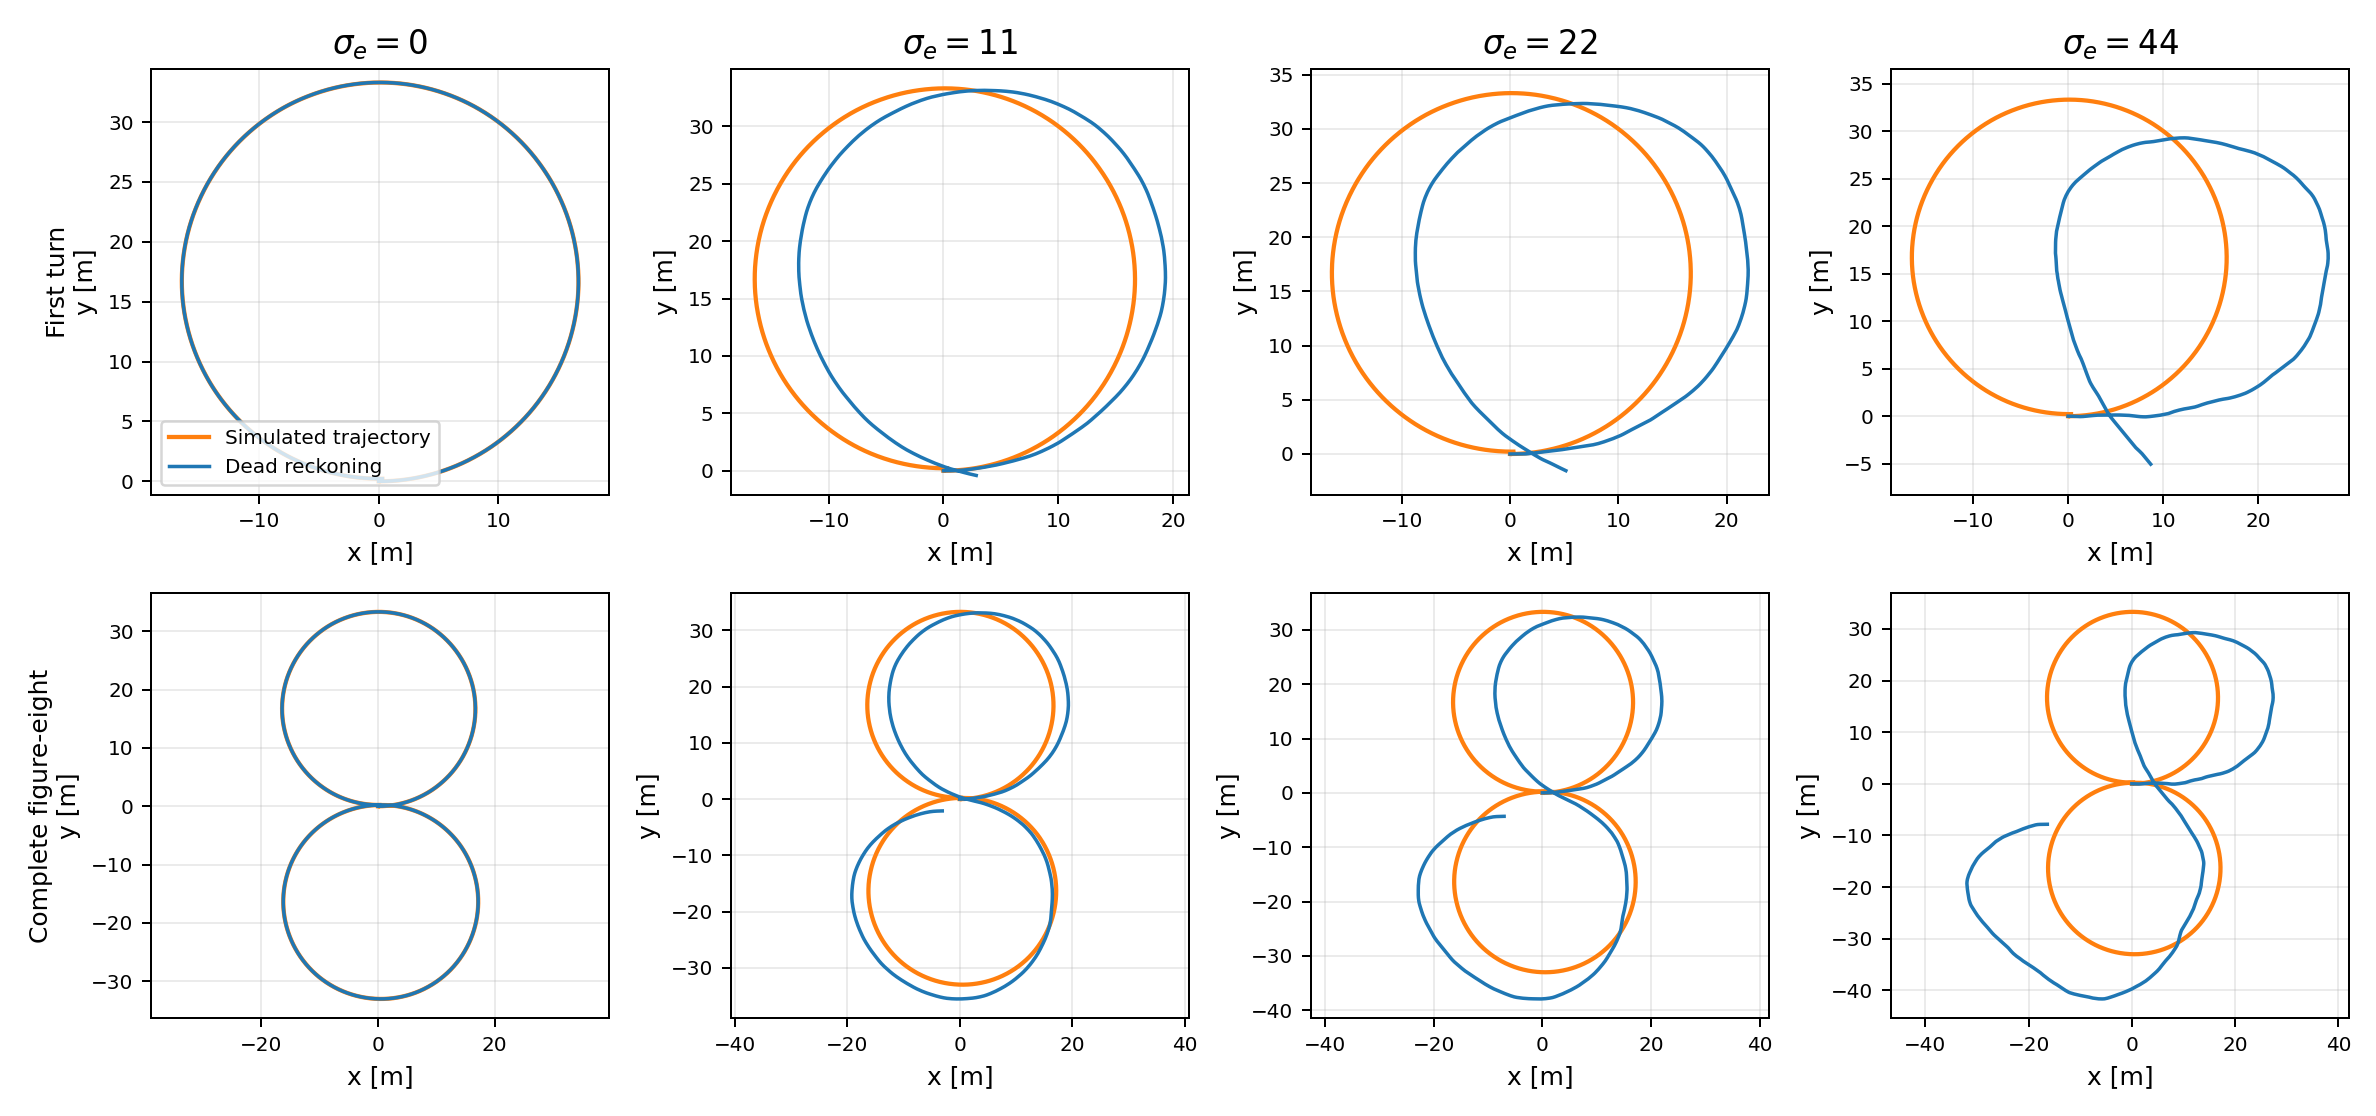
\includegraphics[width=0.94\textwidth]{encoder_trajectory_comparison.png}
    \caption{Simulated and dead-reckoning trajectories for the four tested
    encoder-noise levels.}
    \label{fig:encoder-trajectories}
\end{figure}

With $\sigma_e=0$, the simulated and estimated trajectories practically
overlap. A small separation appears with 11 pulses, becomes clear at the
nominal value of 22 pulses, and strongly deforms the estimate at 44 pulses.
The smallest noise gives the closest result, while 22 pulses is retained as
the nominal sensor setting. This comparison also shows that encoder noise has
a much clearer influence on dead reckoning than the tested values of $K$.

\section{Conclusions}
\label{sec:conclusions}

The two laboratories establish a complete chain from planar rigid-body
kinematics to simulated sensing and odometric localization. The
\texttt{Pose3D} class provides consistent direct and inverse compounding,
which is then reused by both the simulator and estimator. The
differential-drive simulator generates noisy motion and encoder pulses, while
the dead-reckoning class converts those pulses into incremental body motion and
propagates the pose estimate. Circular and opposite-turn tests verify the
expected robot motion and also demonstrate the fundamental limitation of dead
reckoning: without an absolute observation, encoder noise produces
unbounded drift.

\section*{Resources}

The source code used for these laboratories is publicly available in the
\href{https://github.com/Mariolopez31/PR-3501MO3352_2026/tree/main/Lab1-2}%
{Lab 1--2 GitHub directory}:

\noindent\url{https://github.com/Mariolopez31/PR-3501MO3352_2026/tree/main/Lab1-2}

\end{document}
